\chapter{Estendendo a Biblioteca Digital do Participa}
\label{cap:extbibparticipa}

Em função das manifestações sociais que circulam pelo País, o Participa tem sido considerado como uma plataforma estratégica para o Governo Federal e há interesse direto na sua divulgação e uso \footnote{Veja declaração da Presidente Dilma sobre a importância do Participa no contexto do Governo Federal, no endereço: \url{https://www.youtube.com/watch?v=WOLXKzVSZFkt=92m56s}, feito em 23 de maio de 2014.}, com disponibilização de conteúdos que beneficiam os canais formais e informais. Percebe-se ainda que esse portal pode ser entendido como um espaço de colaboração semântico e  social, como está ilustrado na figura \ref{fig:semanticoparticipa}, seguindo as tendências da web semântica e suas tecnologias associadas, além das ferramentas de comunicação social disponíveis.

\graphicspath{{figuras/}}
\begin{figure}[H]
\centering
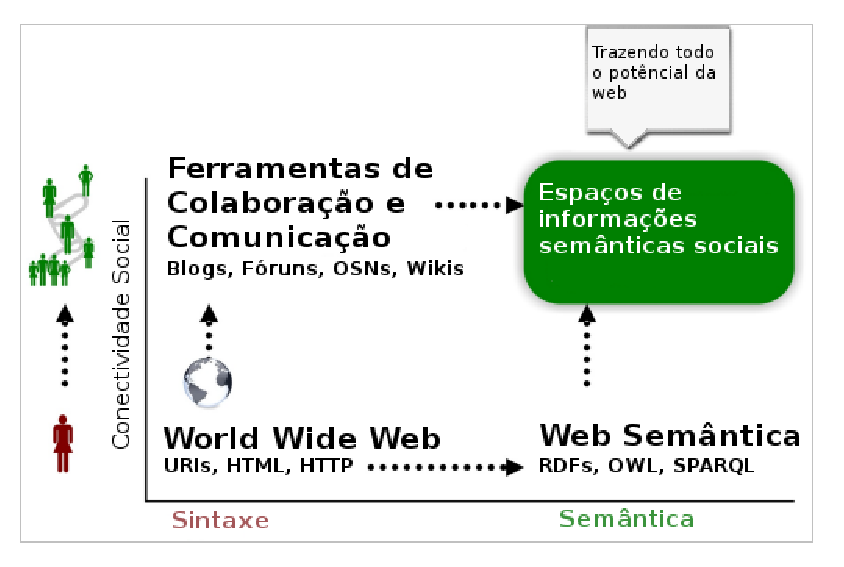
\includegraphics[width=0.9\textwidth]{semantico_participa}
\caption[Espaço de colaboração semântico e social no Participa.br]{Espaço de colaboração semântico e social no Participa.br. Adaptado de \cite{kruk2006libraries}}
\label{fig:semanticoparticipa}
\end{figure}
%Figura 4.1 – Espaço de colaboração semântico e social no Participa.br
%Fonte: Adaptado de Kruk (2006)

Nessa figura, presume-se a utilização do portal dentro do conceito da web 2.0 que é caracterizada por interatividade com o usuário por meio de blogs, wikis, redes sociais online e outros mecanismos descentralizados e interoperáveis. Na perspectiva da web semântica, esses mecanismos de interatividade são aprimorados com a inserção de significados aos conteúdos de informação, permitindo maior interoperabilidade dentro dos canais de comunicação e entre eles, formando um espaço de informação social e semântico. Ao que parece, esse espaço de colaboração social já estava concebido em função das consultorias PNUD contratadas e das discussões identificadas sobre aspectos tecnológicos e metodológicos voltados para a democracia participativa. No entanto, cabem aqui algumas observações para garantir a sua concretização.

No que se refere ao suporte à participação social, é importante que se abram discussões sobre as propostas metodológicas feitas por \cite{solagna2014metodologias} a fim de que essas possam ser refinadas e devidamente aproveitadas como referencial não apenas para construção ou adoção de ferramentas de apoio à participação social disponíveis no portal, mas que tenham impacto na própria concepção ou redesenho da plataforma Participa. Nesse sentido, sugere-se a elaboração de uma agenda de trabalho compatibilizando o tempo hábil para maturação dos processos metodológicos com o desenvolvimento do Noosfero.

De forma similar, é importante que as contribuições feitas por \cite{fabbri2014ontologias} sejam consideradas nas evoluções do Noosfero a fim de aproveitar as definições conceituais da ontologia de participação social para permitir um arcabouço conceitual consolidado e, ao mesmo tempo, garantir a interoperabilidade das informações do Participa com outros ambientes digitais de participação social. A forma de aproveitamento das contribuições da ontologia e dos formatos adotados (como o RDF, por exemplo) deve, portanto, ficar melhor evidenciada junto à coordenação do Portal e da equipe de desenvolvimento do Noosfero.

Seguindo a mesma linha de raciocínio, o formato proposto para organização e catalogação dos conteúdos sobre participação social proposto aqui (vide Capítulo \ref{cap:bibparticipabr}) pode ser integrado com as demais soluções, pela concepção de uma biblioteca digital semântica social, que é mais abrangente que uma biblioteca digital tradicional, conforme está ilustrado na figura \ref{fig:contextoevolutivo}.

\graphicspath{{figuras/}}
\begin{figure}[H]
\centering
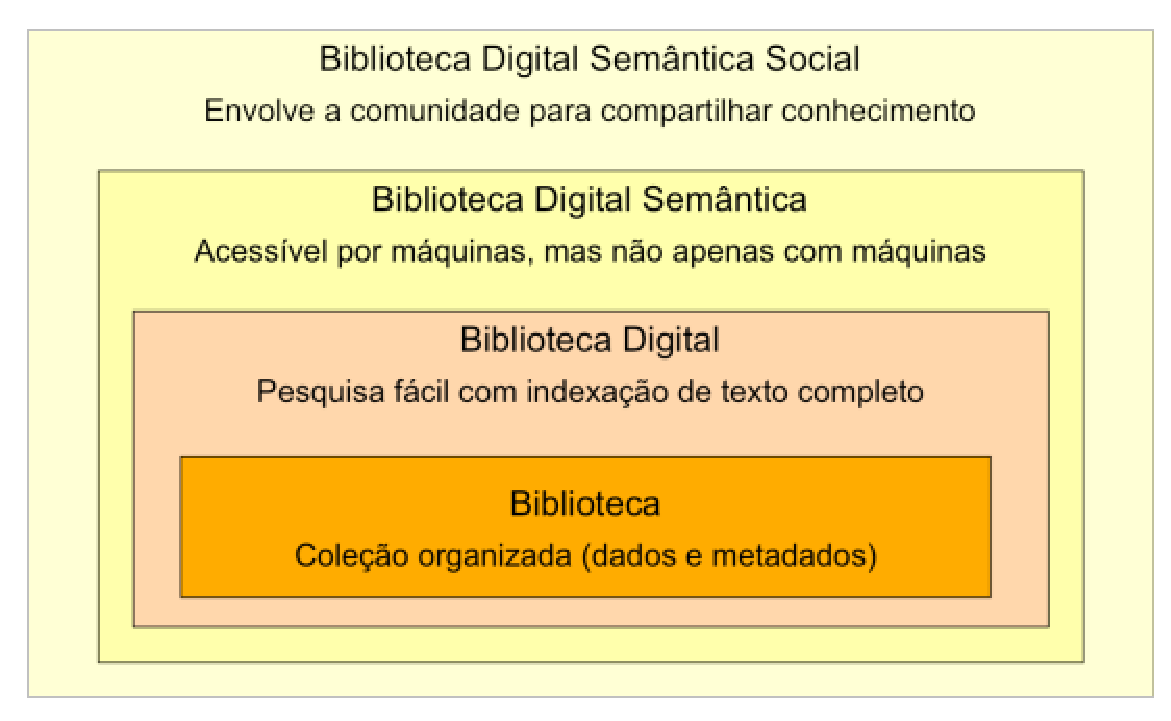
\includegraphics[width=0.8\textwidth]{contexto_evolutivo}
\caption[Contexto evolutivo das bibliotecas]{Contexto evolutivo das bibliotecas. Adaptado de \cite{kruk2006libraries}}
\label{fig:contextoevolutivo}
\end{figure}
%Figura 4.2 – Contexto evolutivo das bibliotecas
%Fonte: Adaptado de kruk (2006)

Portanto, os conteúdos de informação podem ser catalogados em esquemas similares aos que são feitos em bibliotecas tradicionais, mas podem evoluir para conteúdos disponibilizados em bibliotecas digitais semânticas e sociais, ampliando a qualidade do serviço de referência pensado inicialmente. Dessa forma, os conteúdos de informação sobre participação social estariam organizados e a solução de disponibilização de conteúdos seria mais ampla e compatível com as demais consultorias PNUD em andamento.

Segundo \cite{kruk2008semantic}, as bibliotecas digitais semânticas (i) integram informação baseada em diferentes metadados, tais como recursos, profiles de usuário, bookmarks e taxonomias, (ii) provêem interoperabilidade com outros sistemas (não apenas bibliotecas digitais) tanto no nível dos metadados como no nível da comunicação direta, e (iii) provêem interfaces de navegação e pesquisa  mais amigáveis e mais robustas do que as bibliotecas tradicionais.

De fato, no estado da arte das bibliotecas digitais, os usuários são meros consumidores que recuperam conteúdos baseados em registros bibliográficos atualizados (como está proposto no Capítulo \ref{cap:bibparticipabr}), enquanto que nas bibliotecas digitais semânticas e sociais os usuários contribuem efetivamente enriquecendo os objetos digitais com anotações, recomendações e marcações sobre conteúdos de interesse. Nesse contexto, é possível a realização de busca e filtragem colaborativa para facilitar a localização de informações relevantes para os membros da comunidade num contexto mais dinâmico para troca de informações.

Nessa perspectiva, pode-se pensar na utilização de uma abordagem baseada em web semântica para descrição dos objetos de informação e a gestão de conteúdos e inclusão de metadados feita com auxílio da própria comunidade de usuários, nos moldes do que ocorre em softwares como o Connetea (já desativado)\footnote{Informações disponíveis em \url{http://en.wikipedia.org/wiki/Connotea}.}, o Flickr\footnote{Informações disponíveis em \url{https://www.flickr.com/}.}, o CiteULike\footnote{Ver mais informações em \url{http://www.citeulike.org/}.}, o del.icio.us\footnote{Informações adicionais em \url{http://en.wikipedia.org/wiki/Connotea}.} e o ReadCube\footnote{Ver maiores informações em \url{http://www.citeulike.org/}.} Esses ambientes incluem a gestão de blogs, onde os usuários podem salvar links para seus sites favoritos, podem compartilhar essas marcações, além de RSS feeds e demais anotações realizadas sobre conteúdos de interesse. Essa estratégia permite que  usuários possam trilhar informações de participação social postadas sobre uma determinada tag ou encontrar usuários com interesses similares, aumentando a interatividade entre os membros da comunidade.

Com a inserção de aspectos semânticos, o ambiente pode inferir ou reconhecer sites relacionados à participação social e coletar metadados automaticamente para um artigo ou página que está sendo marcado no momento do uso. Nesse esquema, a plataforma poderia reconhecer quais metadados os usuários inseriram para os sites que visitaram e essa informação poderia ser compartilhada com os demais e gerar novas informações sobre sites ou materiais potencialmente relacionados.

Ainda com relação ao tema de bibliotecas digitais, foram feitos estudos preliminares sobre alguns softwares livres que poderiam ser utilizados, cujas descrições resumidas estão no Anexo \ref{Att:anexobibliotecas} deste documento. Um dos softwares analisados é o JeromeDL\footnote{Recuperado do endereço \url{http://sourceforge.net/projects/jeromedl/}}, que chamou a atenção pelo fato de ser compatível com bibliotecas digitais semânticas e, além disso, contemplar o SIOC - uma ontologia de participação social (Semantically-Interlinked Online Communities Project\footnote{Veja maiores informações em \url{http://www.sioc-project.org/}} - que provê possibilidades de interconexão de discussões promovidas por canais como blogs e fóruns, dentre outros.

Além de ser um espaço de colaboração social, é interessante que o portal seja também um ambiente de monitoramento de demandas sociais para permitir recuperar informações importantes para elaboração de políticas sociais mais compatíveis com as demandas mais emergentes identificadas. Para essa funcionalidade, uma alternativa interessante é a adoção de uma variante do produto denominado Radar Eletrônico\footnote{Maiores informações em \url{http://www.radareleitoral.com.br/}}, que é um software para monitoramento de opiniões sobre candidatos e partidos políticos, ou a construção de um módulo de monitoramento dentro do próprio Participa.

As ideias apresentadas aqui estão num estágio inicial e precisam ser consideradas dentro daquilo que se deseja como futuro para o Participa, verificando em que medida podem ser incorporadas no Portal. Mesmo com esses levantamentos prévios, é importante que sejam feitas novas avaliações sobre o que foi proposto e realizar reuniões de alinhamento com os consultores PNUD, com a equipe de desenvolvimento Noosfero e com a coordenação do Portal para um debate acerca dessas possibilidades a fim de se traçar um caminho de futuro para o portal Participa.
